\section{Introduction}\label{sec:intro}
\fixme{Review}

Filtering operations are often a crucial step of image processing and a particular sub-group of these are edge-aware smoothing filters. 
They are used as a basic building block for multiple other applications.
For example, such filters can be used to extract or remove features from an
image, to colorize the image in a intuitive fashion by colouring specific
items on an image, or to perform other tasks such as noise removal and
image compression ~\cite{GastalOliveira2011DomainTransform}.

As in most cases with image (and in particular with video) processing, it is highly required that the filters have a low computational cost and therefore can produce fast results. This is desireable to allow for real-time transformation of video streams as well as immediate feedback during image editing and in general when working on large datasets. 
It is also true that image recording technologies advance and therefore can create images of greater resolution, which means an increase in
the amount of computation needed for filtering.

\setlength\fboxsep{0pt}
\setlength\fboxrule{0.5pt}
 
\begin{figure}\vspace{-1mm}
  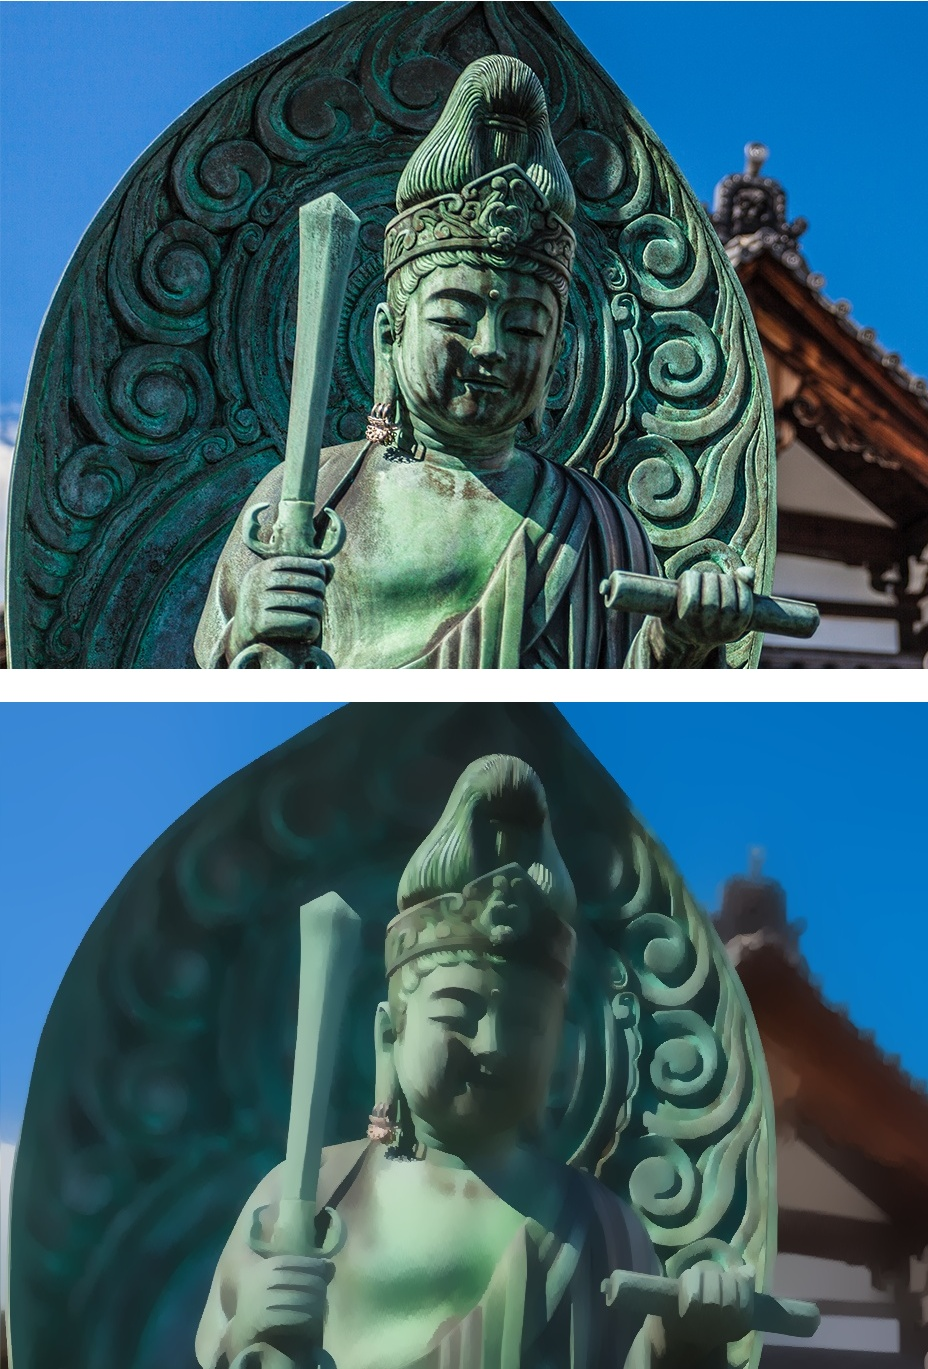
\includegraphics[trim=-30mm 0mm 0mm 0mm, clip, width=0.37\textwidth]{figures/input_output}
  \caption{Example input and output of our Normalized convolution implementation.\label{performance}}
\end{figure}


There exist multiple algorithms that perform this type of filtering, most of which fall into the categories of \textit{Bilateral filtering} and \textit{Anisotropic diffusion}. However most of these suffer either from quality, performance or scalability drawbacks. Moreover, some of them only support grayscale images.

Recently, a new method that promises to solve these problems was prososed by Eduardo S. L. Gastal and Manuel M. Oliveira in their paper \textit{Domain Transform for Edge-Aware Image and Video Processing} ~\cite{GastalOliveira2011DomainTransform}.

This publication gives an in depth explanation of the theoretical foundations of the technique as well as presenting three different implementation approaches. These three approaches are called \textit{Normalized convolution} (NC), \textit{Interpolated convolution} (IC) and \textit{Recursive filtering} (RF).

So far the only publicly available implementation of these methods is done in MATLAB, published on the original papers homepage. While useful for verification and demonstration purposes, its runtime performance is far from optimal. The work presented here aims at providing an optimized implementation of the \textit{Normalized convolution} variant of the algorithm on the CPU while documenting the optimization process. We have implemented the algorith in C/C++ and proceeded to use the techniques described in the \textit{How to Write Fast Numerical Code} course ~\cite{HowToFastNumCode:2013:Webpage} to improve its performance.

\comment{Do not start the introduction with the abstract or a slightly modified
version. It follows a possible structure of the introduction. 
Note that the structure can be modified, but the
content should be the same. Introduction and abstract should fill at most the first page, better less.

\mypar{Motivation} The first task is to motivate what you do.  You can
start general and zoom in one the specific problem you consider.  In
the process you should have explained to the reader: what you are doing,
why you are doing, why it is important (order is usually reversed).

For example, if my result is the fastest DFT implementation ever, one
could roughly go as follows. First explain why the DFT is important
(used everywhere with a few examples) and why performance matters (large datasets,
realtime). Then explain that fast implementations are very hard and
expensive to get (memory hierarchy, vector, parallel). 

Now you state what you do in this paper. In our example: 
presenting a DFT implementation that is
faster for some sizes than all the other ones.

\mypar{Related work} Next, you have to give a brief overview of
related work. For a paper like this, anywhere between 2 and 8
references. Briefly explain what they do. In the end contrast to what
you do to make now precisely clear what your contribution is.
}